\subsubsection{Word Mover's Distance} % (fold)
\label{sub:own_wmd}
As mentioned in \autoref{sub:word_movers_distance}, the document or sentence wise similarity can not be captured fully using word vectors only. In our last approach, we therefore use WMD to again cluster the dataset. To calculate the distance between sentences with WMD, the sentences have to be represented by their word embeddings. Hence, we reuse the word vectors we created with the aforementioned word2vec models. Instead of a word based distance, we now create a distance matrix $D\in\mathbb{R}^{n\times n}$, with $n$ being the total number of sentences, as follows:
\begin{enumerate}
	\item For every sentence in the \crowdre{} corpus, calculate the distances to every other sentence using WMD.
	\item Save the distances in the matrix $D$, as shown in \autoref{fig:embeddings_matrices} (3).
\end{enumerate}
We then cluster the sentences by applying K-Means to the resulting matrix $D$. 
As $D$ is 2-dimensional already, there is no need to reduce its dimensions before.

 \begin{figure}[ht]
  \begin{center}
    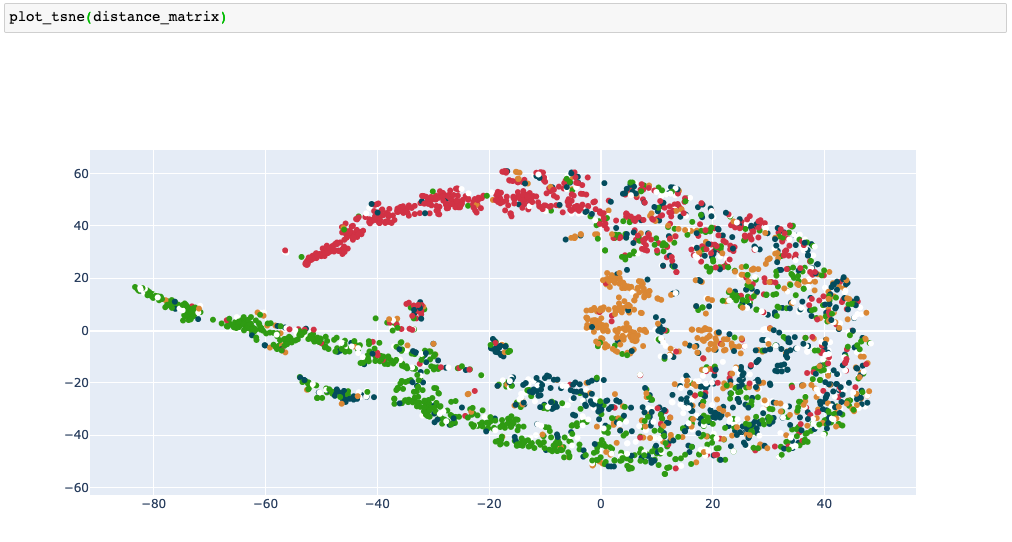
\includegraphics[width=\textwidth]{screenshots/our_word_movers_distance_tsne.png}
    \caption{Distance Matrix of the Word Mover's Distance with a self-trained model (plotted with t-SNE)}
    \label{fig:wmd-selftrained-1}
  \end{center}
\end{figure}
\FloatBarrier